% This file was created with tikzplotlib v0.10.1.
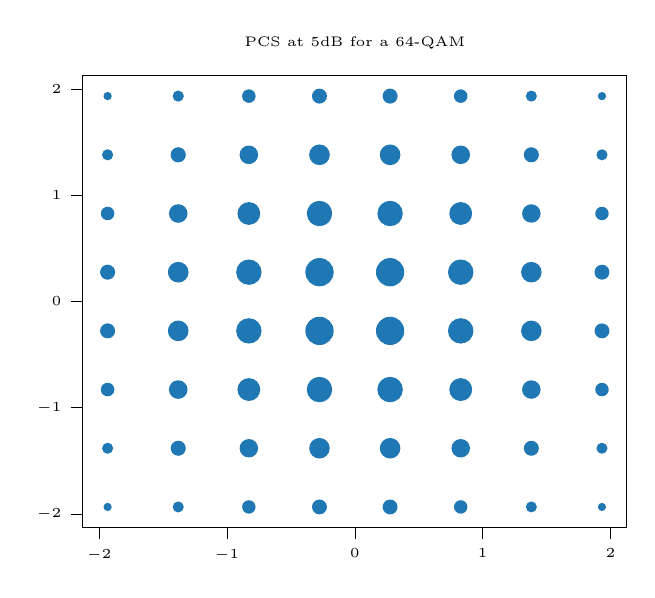
\begin{tikzpicture}[font=\tiny]

\definecolor{darkgray176}{RGB}{176,176,176}
\definecolor{steelblue31119180}{RGB}{31,119,180}

\begin{axis}[
width=0.7\columnwidth,
tick align=outside,
tick pos=left,
title={PCS at 5dB for a 64-QAM},
x grid style={darkgray176},
xmin=-2.12673020362854, xmax=2.12673020362854,
xtick style={color=black},
y grid style={darkgray176},
ymin=-2.12673020362854, ymax=2.12673020362854,
ytick style={color=black}
]
\addplot [
  draw=steelblue31119180,
  fill=steelblue31119180,
  mark=*,
  only marks,
  scatter,
  scatter/use mapped color={
	    draw=steelblue31119180,
	    fill=steelblue31119180,
	  },
  scatter/@pre marker code/.append style={/tikz/mark size=\perpointmarksize},
  visualization depends on={\thisrow{sizedata} \as\perpointmarksize}
]
table{%
x  y  sizedata
-1.93339109420776 1.93339109420776 1.280015
-1.38099372386932 1.93339109420776 1.8017671
-0.828596234321594 1.93339109420776 2.2371068
-0.276198744773865 1.93339109420776 2.5059946
0.276198744773865 1.93339109420776 2.5063868
0.828596234321594 1.93339109420776 2.2430263
1.38099372386932 1.93339109420776 1.7893766
1.93339109420776 1.93339109420776 1.2696476
-1.93339109420776 1.38099372386932 1.8017671
-1.38099372386932 1.38099372386932 2.536193
-0.828596234321594 1.38099372386932 3.1489832
-0.276198744773865 1.38099372386932 3.5274734
0.276198744773865 1.38099372386932 3.5280254
0.828596234321594 1.38099372386932 3.1573153
1.38099372386932 1.38099372386932 2.5187516
1.93339109420776 1.38099372386932 1.787174
-1.93339109420776 0.828596234321594 2.2371068
-1.38099372386932 0.828596234321594 3.1489832
-0.828596234321594 0.828596234321594 3.9098349
-0.276198744773865 0.828596234321594 4.3797755
0.276198744773865 0.828596234321594 4.3804607
0.828596234321594 0.828596234321594 3.92018
1.38099372386932 0.828596234321594 3.127328
1.93339109420776 0.828596234321594 2.2189877
-1.93339109420776 0.276198744773865 2.5059946
-1.38099372386932 0.276198744773865 3.5274734
-0.828596234321594 0.276198744773865 4.3797755
-0.276198744773865 0.276198744773865 4.9061995
0.276198744773865 0.276198744773865 4.9069676
0.828596234321594 0.276198744773865 4.391364
1.38099372386932 0.276198744773865 3.503215
1.93339109420776 0.276198744773865 2.4856977
-1.93339109420776 -0.276198744773865 2.5063868
-1.38099372386932 -0.276198744773865 3.5280254
-0.828596234321594 -0.276198744773865 4.3804607
-0.276198744773865 -0.276198744773865 4.9069676
0.276198744773865 -0.276198744773865 4.907736
0.828596234321594 -0.276198744773865 4.392051
1.38099372386932 -0.276198744773865 3.5037634
1.93339109420776 -0.276198744773865 2.4860866
-1.93339109420776 -0.828596234321594 2.2430263
-1.38099372386932 -0.828596234321594 3.1573153
-0.828596234321594 -0.828596234321594 3.92018
-0.276198744773865 -0.828596234321594 4.391364
0.276198744773865 -0.828596234321594 4.392051
0.828596234321594 -0.828596234321594 3.9305527
1.38099372386932 -0.828596234321594 3.1356027
1.93339109420776 -0.828596234321594 2.224859
-1.93339109420776 -1.38099372386932 1.7893766
-1.38099372386932 -1.38099372386932 2.5187516
-0.828596234321594 -1.38099372386932 3.127328
-0.276198744773865 -1.38099372386932 3.503215
0.276198744773865 -1.38099372386932 3.5037634
0.828596234321594 -1.38099372386932 3.1356027
1.38099372386932 -1.38099372386932 2.5014305
1.93339109420776 -1.38099372386932 1.7748837
-1.93339109420776 -1.93339109420776 1.2696476
-1.38099372386932 -1.93339109420776 1.787174
-0.828596234321594 -1.93339109420776 2.2189877
-0.276198744773865 -1.93339109420776 2.4856977
0.276198744773865 -1.93339109420776 2.4860866
0.828596234321594 -1.93339109420776 2.224859
1.38099372386932 -1.93339109420776 1.7748837
1.93339109420776 -1.93339109420776 1.2593642
};
\end{axis}

\end{tikzpicture}
